
%(BEGIN_QUESTION)
% Copyright 2011, Tony R. Kuphaldt, released under the Creative Commons Attribution License (v 1.0)
% This means you may do almost anything with this work of mine, so long as you give me proper credit

Suppose this Fisher model 546 I/P transducer has an input range of 4-20 mA and an output range of 3-15 PSI:

$$\includegraphics[width=15.5cm]{i03937x01.eps}$$

Identify which way the magnetic shunt would have to be moved in order to re-calibrate the I/P transducer to a new output range of 4-20 PSI (from 3-15 PSI), explaining your reasoning.

\vskip 10pt

Identify which way the zero screw would have to be turned in order to re-calibrate the I/P transducer to a new output range of 2-14 PSI (from 3-15 PSI), explaining your reasoning.

\vskip 20pt \vbox{\hrule \hbox{\strut \vrule{} {\bf Suggestions for Socratic discussion} \vrule} \hrule}

\begin{itemize}
\item{} What would happen if some of the turns in the electromagnet coil were shorted past?  Would this cause a {\it zero} shift, a {\it span} shift, or a {\it linearity} shift?
\item{} What would happen if the zero spring broke into two separate pieces?  Would this cause a {\it zero} shift, a {\it span} shift, or a {\it linearity} shift?
\item{} Suppose this I/P outputs a pressure of 9.0 PSI at an input current of 12.3 mA.  Calculate the error, {\it in percent of span}.
\item{} Suppose this I/P outputs a pressure of 12.5 PSI at an input current of 16.0 mA.  Calculate the error, {\it in percent of span}.
\item{} Suppose this I/P outputs a pressure of 5.7 PSI at an input current of 8.0 mA.  Calculate the error, {\it in percent of span}.
\end{itemize}

\underbar{file i03937}
%(END_QUESTION)





%(BEGIN_ANSWER)

Move the magnetic shunt {\it further out} in order to re-calibrate from 3-15 PSI to 4-20 PSI.

\vskip 10pt

Turn the zero screw so the spring doesn't push down as hard on the right-hand side of the beam in order to re-calibrate from 3-15 PSI to 2-14 PSI.

%(END_ANSWER)





%(BEGIN_NOTES)

Since we desire a greater range of output pressure for the same range of input current as before, this requires an amplification of magnetic force.  Moving the shunt further away from the assembly bypasses less magnetic flux, causing the beam to react stronger against the permanent magnet field with the same amount of current.

\vskip 10pt

Since we desire a downward shift in pressure (less pressure) than before, we don't need the zero spring to provide as much bias force as it previously did.  This means we should relax the spring's compression.






\vfil \eject

\noindent
{\bf Summary Quiz:}

Suppose a technician adjusts the screw on this Fisher model 546 I/P transducer so that {\it less} spring force is exerted downward on the beam than before.  Supposing its output calibration used to be 3-15 PSI (for 4-20 mA input signal), identify what the new calibrated output range might be:

$$\includegraphics[width=15.5cm]{i03937x02.eps}$$

\begin{itemize}
\item{} 2-15 PSI
\vskip 5pt 
\item{} 2-14 PSI
\vskip 5pt 
\item{} 3-16 PSI
\vskip 5pt 
\item{} 15-3 PSI
\vskip 5pt 
\item{} 4-16 PSI
\vskip 5pt 
\item{} 4-20 PSI
\end{itemize}


%INDEX% Calibration, pneumatic instrument: zero and span adjustments

%(END_NOTES)


